%********************************************************************************
%       Preamble Information
%********************************************************************************
\documentclass[11pt, twocolumn]{article}
\usepackage[T1]{fontenc}
\usepackage[utf8]{inputenc}
\usepackage{mathpazo}
\usepackage{multicol}
\setlength\columnsep{20pt}

\usepackage{hyperref}
\hypersetup{
    colorlinks=true,
    linkcolor=blue,
    filecolor=magenta,      
    urlcolor=blue,
    citecolor=black
    }
% Used to include graphic images into LaTeX
\usepackage{graphicx}
% Tells the compiler to search in the images/ 
% folder for any included figures
\graphicspath{ {./images/} }

% Make lists more compact
% (from pandoc template)
\providecommand{\tightlist}{\setlength{\itemsep}{0pt}\setlength{\parskip}{0pt}}

% Prevent overfull lines
\setlength{\emergencystretch}{1em}

% No indentation and space between paragraph
\setlength{\parindent}{0.0in}
%\setlength{\parskip}{0.04in}
% Have space between paragraph
\setlength{\parskip}{11pt}

% Margin support
\usepackage[margin=0.75in]{geometry}

% header and footer
\usepackage{fancyhdr}

\newcommand{\thelabnumber}{HW3}
\newcommand{\thetitle}{HW3: Computer History}
% Update this line with your name 
\newcommand{\theauthor}{Jared Martinez \\ Logan Baeza}

% Write title and author
\title{{\large } \thetitle}
\author{\theauthor}
\date{\today}

\pagestyle{fancy}
\fancyhf{}
\fancyfoot[R]{\thepage}
\fancyfoot[C]{HW3}
\fancyfoot[L]{CSE/IT 101 HW3}
\renewcommand{\footrulewidth}{1pt}
\renewcommand{\headrulewidth}{0pt}
\fancypagestyle{firstpage}{%
  \fancyhf{}% clear default for header and footer
  \fancyfoot[R]{\thepage}
  \fancyfoot[C]{HW3}
  \fancyfoot[L]{CSE/IT 101}
  \renewcommand{\footrulewidth}{1pt}
    \renewcommand{\headrulewidth}{0pt}
}

%********************************************************************************
%      Begin Document
%********************************************************************************
\begin{document}
\maketitle

\thispagestyle{firstpage}

%********************************************************************************
%      Report Content
%********************************************************************************
\section{Introduction}
Supercomputers are some of the most intricate, complex, and utterly awe-inspiring technological marvels that humankind has ever created. With the ability to preform millions of calculations in a matter of seconds, these machines have greatly advanced the human understanding of science. Using multiple powerful CPU's, a supercomputer sends signals within itself at almost the speed of light, with the fastest performing a massive 442 quadrillion (\begin{math}4.42x10^1^5)\end{math}) Floating-Point-Operations per Second (FLOPS). By comparison, a standard household computer can only process at a speed of 2.8 billion (\begin{math}2.8x10^9\end{math}) Operations per Second.

\section{Time Period}
The concept of a supercomputer has existed for a remarkably long time in relation to computer history. In 1964, Seymoore Cray was credited for building the Control Data Corporation's CDC 6600, after a brief competition with IBM to build an extremely fast computer. This was the first computer to be dubbed as a supercomputer, with the ability to perform three million FLOPS. Today, the official record holder for the world's fastest supercomputer is Fujitsu Global's Fugaku Supercomputer, which was launched in 2021, with a normal processing speed of 442 quadrillion (\begin{math}4.42x10^1^5\end{math}) Floating-Point-Operations per Second (FLOPS), with the ability to be overclocked to be faster. Research still continues to this day to speed up the computers, but the processes are being controlled by the limitation that data cannot be transferred at a speed above the speed of light.

\section{Computer Hardware}
Supercomputers use the same general hardware as a standard computer, but on a much larger, more powerful scale. Many supercomputers are the size of a whole room, with large cases containing hundreds of thousands of CPU's, GPU's, memory banks, and user peripherals. Supercomputers need this much hardware in order to reach their maximum processing speeds. The Fugaku Supercomputer has a total memory capacity of 4.85 PiB, or 5460615 gB of memory, across three layers of storage systems, and 48 cores dedicated to processing, with 6 additional cores for support. All of this technology did not come cheap, with a total price tag of roughly \$1 Billion USD 

Figure \ref{fig:Fugaku} is a picture of Fugaku in Kobe, Japan.
\begin{figure}
    \centering
    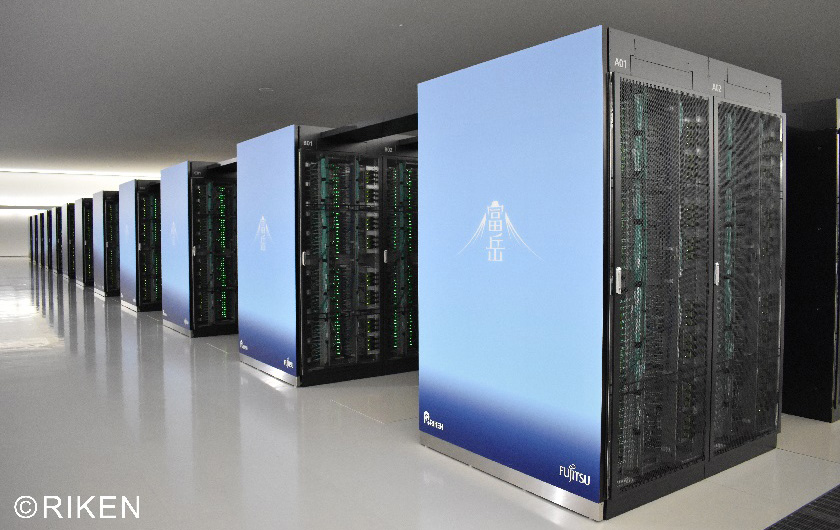
\includegraphics[width=0.45\textwidth]{images/Fugaku.jpg}
    \caption{The Fugaku Supercomputer}
    \label{fig:Fugaku}
\end{figure}

I found this image on the Fugaku Supercomputer webpage \cite{fugaku}. 

\subsection{Computer Software}
Linux is the dominant operating system which almost all 500 supercomputers have. However, each manufacturer optimizes its own Linux derivative to maximize hardware performance.The reason for Linux being the prime OS is because of its open source nature. Supercomputers are specific devices built for specific purposes. This requires a operating system able to be customized to fit those specific needs. Linux, being a free and open sourced operating system would naturally make it a prime candidate for supercomputers because of its flexibility. As for other software, it is extremely hard to get data on the other software used because the purposes and build of supercomputers are so vastly different and diverse.

\subsection{Conclusion}
In conclusion, supercomputers cover a broad range of operations which make them all unique. These are very powerful and fast machines; such that the fastest supercomputer to date can perform a whopping 442 quadrillion FLOPS (\begin{math}4.42x10^1^5\end{math}). The size these machines are approximated to be around 5,600 (\begin{math}ft^2\end{math}). For reference, this is equivalent to about the size of two tennis courts. As of today, there are a little over 500 supercomputers in the world with increasing numbers despite them having an insane cost of anywhere from 30 million to 1 billion US dollars.

%********************************************************************************
%      Report Content
%********************************************************************************
\bibliographystyle{acm}
\bibliography{sources.bib}

\cite{NAS}
\cite{fugaku}
\cite{Brit}
\cite{suse}


\end{document}